\documentclass{book}

%\usepackage[left=1in, right=1in, top=1in, bottom=1in]{geometry} %adjust margins

\usepackage{amsmath, amsfonts, amscd, amsthm, amssymb}
\usepackage{latexsym, verbatim, hyperref, graphicx, epstopdf}
\usepackage{tikz}

\renewcommand{\emptyset}{\varnothing}

%Matching numbering to the book:
\usepackage{tipa}

\renewcommand\thepart{\arabic{part}}
\renewcommand\thechapter{\Roman{chapter}}
\renewcommand\thesection{\arabic{section}}
\renewcommand\thesubsection{[\thesection\textceltpal\arabic{subsection}]} %needed tipa package for \textceltpal

\newtheorem{majorEx}{}[section]
\renewcommand{\themajorEx}{\thesection.\Alph{majorEx}}
\newcommand{\centerimage}[1]{\vcenter{\hbox{#1}}}

\newtheorem{minorEx}{}[section]
\renewcommand{\theminorEx}{\thesection.\arabic{minorEx}}
%%%%%%%%%%%%%%%%%%%%%%%%%%%%%%%%%%%%%%%%%%%%%%%%%%%%%%%%%%%%
%Fixing a ToC spacing issue:
\usepackage{tocloft}
\addtolength{\cftchapnumwidth}{10pt}%add some space to make room between the chapter numerals and chapter title
%%%%%%%%%%%%%%%%%%%%%%%%%%%%%%%%%%%%%%%%%%%%%%%%%%%%%%%%%%%%
%Macros:
%mathbb of usefull characters, for natural numbers, integers, reals, rationals, complex
\newcommand{\NN}{\mathbb{N}}
\newcommand{\ZZ}{\mathbb{Z}}
\newcommand{\RR}{\mathbb{R}}
\newcommand{\QQ}{\mathbb{Q}}
\newcommand{\CC}{\mathbb{C}}
%%%%%%%%%%%%%%%%%%%%%%%%%%%%%%%%%%%%%%%%%%%%%%%%%%%%%%%%%%%%

\title{Workbook for MAT331-Topology}
\date{Fall 2016}
\author{This workbook, part of the coursework for MAT331-Topology, is based on \cite{viro}.}


\begin{document}
	%\maketitle
	%\tableofcontents
	%%
	%%
	%%
	%\part{General Topology}
	
	\chapter{Structure and Spaces}
		\section{Set-Theoretic Digression: Sets}
			\subsection{Sets and Elements}%1'1
			\subsection{Equality of Sets}%1'2
			\subsection{The Empty Set}%1'3
			\subsection{Basic Set of Numbers}%1'4
			\subsection{Describing a Set By Listing Its Elements}%1'5
				\begin{minorEx}%1.1
					What is $ \{\emptyset\} $? How many elements does it contain?
				\end{minorEx}
				\begin{proof}[Answer]
					This is a set made up of the empty set, it contains one element.
				\end{proof}
				\begin{minorEx}%1.2
                Which of the following formulas are correct:
				\begin{enumerate}
                \item $\emptyset \in \{\emptyset, \{\emptyset\}\}$ is correct
                \item $\{\emptyset\} \in \{\{\emptyset\}\}$ is correct
                \item $\emptyset \in \{\{\emptyset\}\}$ is incorrect
                \end{enumerate}
                Primary author: Willie Kaufman
				\end{minorEx}
				\begin{minorEx}%1.3
					Yes, \{\{$\emptyset$\}\} contains just one element. \newline
                    Primary author: Willie Kaufman
				\end{minorEx}
				\begin{minorEx}%1.4
					How many elements do the following sets contains?
				\end{minorEx}
                \begin{enumerate}
					\item $\{1,2,1 \}$; 2 elements
					\item $\{ 1,2,\{1,2\} \}$; 3 elements
					\item $\{\{ 2 \} \}$; 1 element
					\item $\{ \{1 \}, 1\}$; 2 elements
					\item $\{ 1, \emptyset \}$; 2 elements
					\item $\{ \{ \emptyset \}, \emptyset \}$; 2 elements
					\item $\{ \{ \emptyset\}, \{\null\} \}$; 1 element
					\item $\{x, 3x-1 \} for x\in \RR$; 1 element if $x = \frac{1}{2}$, and 2 elements for all for all values of $x$
                \end{enumerate}
                \begin{minorEx}
                (a) : $\{0, 1, 2, 3, 4\}$
                
                (b) : $\emptyset$
                
                (c) : $\{-1, -2, -3, \cdots\}$
                \end{minorEx}
			\subsection{Subsets}%1'6
				\begin{majorEx}%1.A
					Let a set $ A $ have $a$ elements, and let a set $B$ have $b$ elements. Prove that if $A \subset B $, then $a\leq b$.
				\end{majorEx}
				\begin{proof}
					Suppose  $ A $ is a set made up of $a$ elements, and $B$ is a set made up of $b$ elements. Suppose $a > b$; then there must be some element $x \in A$ that satisfies $x \notin B$. This implies that $A \not\subset B$, as $x$ is not a member of $B$. By the contrapositive, we obtain the desired result.
				\end{proof}
			\subsection{Properties of Inclusion}%1'7
				\begin{majorEx}[Reflexivity of Inclusion]%1.B
                Any set includes itself: $A \subset A$ holds true for any $A$.

Proof: We first let $A$ be an arbitrary Set. Suppose that $A$ is the empty set. We would then see that as $A$ doesn't have any elements, that it is vacuously true that every element of $A$ is in $A$, and thus  $A \subset A$. Now suppose that $A$ is non empty. Let $a \in A$ be arbitrary. We see that $a \in A$, and as $a$ was arbitrary, we know that this is true for all elements of $A$, and thus $A \subset A$. As $A$ was arbitrary, and $A \subset A$ for all cases, we see that $A \subset A$ holds true for any $A$.
				\end{majorEx}
				\begin{majorEx}%1.C
					\textbf{\textit{The Empty Set Is Everywhere.}} The inclusion $\emptyset \subset A$ holds true for any A. In other words, the empty set is present in each set as a subset.
                    \begin{proof}
                    Assume that $\emptyset \subset A$ does not hold, by defintion of inclusion, there exist at least one element $a \in \emptyset$ such that $a \not\in A$. Since $\emptyset$ does not contain any element, we have a contradiction.
                    \end{proof}
				\end{majorEx}
				\begin{majorEx}%1.D
					If A , $B$, and $C$ are sets, $A \subset B$, and $B \subset C$, then $A \subset C$. 
				\end{majorEx}
                \begin{proof}
                Let $A$, $B$, and $C$ be arbitrary sets such that $A \subset B$ and $B \subset C$. If $A$ is the empty set, it is true that $A \subset C$. If $A$ is nonempty, choose an arbitrary element $a \in A$. Because $A \subset B$, we know that $a \in B$, and similarly because  $B \subset C$, $a \in C$. Since $a$ was arbitrary, $A \subset C$. \newline
                \end{proof}
      		 Primary author: Willie Kaufman
			\subsection{To Prove Equality of Sets, Prove Two Inclusions}%1'8
            	\begin{majorEx} % 1.E
                	[Criterion of Equality for Sets.]
                    $A = B$ if and only if $A \subset B$ and $B \subset A$.
                \end{majorEx}
                \begin{proof}
					Let $A$ and $B$ be arbitrary sets. Let us first suppose that $A = B$. We show that $A \subset B$ and $B \subset A$. Let $x \in A$ be arbitrary. Since $A = B$, they have the same elements; since $x$ is an element of $A$, $x$ is an element of $B$. Hence, $A \subset B$. A similar argument establishes that $B \subset A$.
                    
                    We now establish the converse of the previous claim via contraposition. Suppose that it is not the case that $A \subset B$ and $B \subset A$; without loss of generality, we shall assume that $A \not\subset B$. Then there necessarily exists an element $x \in A$ satisfying $x \notin B$. As such, it is not the case that $A$ and $B$ contain the same elements, since $B$ does not contain $x$. Hence, $A \ne B$. By the contrapositive, this establishes the converse.
				\end{proof}
			\subsection{Inclusion Versus Belonging}%1'9
            \begin{majorEx}%1.F
            $x \in A$ if and only if $\{x\} \subset A$.
            \end{majorEx}

\begin{proof} We will first show that if $\{x\} \subset A$, then $x \in A$. We can see that as $\{x\}$ is a set described by listing all of its elements, that $x \in \{x\}$. We also see that
as $\{x\} \subset A$, that all of the elements of $\{x\}$ are also elements of $A$, and thus $x \in A$. We thus know that if $\{x\} \subset A$, then $x \in A$.

We will now show that if $x \in A$, then $\{x\} \subset A$. We can see that as $\{x\}$ is a set described by listing all of its elements, that $x$ is the only element in $\{x\}$.
We also see that as $x \in A$, that all elements of $\{ x\}$ belong to $A$, and thus $\{x\} \subset A$. We now can see that $x \in A$ if and only if $\{x\} \subset A$.
\end{proof}
			
            \begin{majorEx}%1.G
            \textbf{\textit{Non-Reflexivity of Belonging.}} Construct a set $A$ such that $A \not\in A$.
            \newline $\{1\} \not\in \{1\}$
            \end{majorEx}
            
            \begin{majorEx}%1.H
            \textbf{\textit{Non-Transitivity of Belonging.}} Construct three sets A, B, and C such that $A \in B$ and $B \in C$, but $A \not \in C$.
            \newline $A = \{1\}$
            \newline $B = \{\{1\}, 2\}$
            \newline $C = \{\{\{1\}, 2\}, 3\}$
            \end{majorEx}
            
			\subsection{Defining a Set by a Condition (Set-Builder Notation)}%1'10
            
            
			\subsection{Intersection and Union}%1'11
            
            \begin{majorEx} % 1.I
            [Commutativity of $\cap$ and $\cup$]
            For any two sets $A$ and $B$, we have
            \[
            A \cap B = B \cap A \quad \text{and} \quad
            A \cup B = B \cup A.
            \]
            \end{majorEx}
            \begin{proof}
            For our proof we rely on the commutativity of logical operators. Namely, we have
            \[
            \alpha \land \beta = \beta \land \alpha \quad \text{and} \quad
            \alpha \lor \beta = \beta \lor \alpha, 
            \]
            where $\alpha$ and $\beta$ are arbitrary statements.
            
            Let $A$ and $B$ be arbitrary sets. Then $x \in A \cap B$ if and only if $x \in A$ and $x \in B$, which holds if and only if $x \in B$ and $x \in A$, which holds if and only if $x \in B \cap A$. This establishes via double-containment that $A \cap B = B \cap A$.
            
            Similarly, $x \in A \cup B$ if and only if $x \in A$ or $x \in B$, which holds if and only if $x \in B$ or $x \in A$, which holds if and only if $x \in B \cup x \in A$. This establishes via double-containment that $A \cup B = B \cup A$.
            \end{proof}
            
            \begin{minorEx}%1.6
            Prove that for any set $A$ we have $ A \cap A = A$, $A \cup A = A$, $A \cup \emptyset = A$, and $A \cap \emptyset = \emptyset$.
            \begin{proof}
            Let $A$ be an arbitrary set. If $A$ is the empty set, each of these is true. So we consider when A is not the emptyset. Choose an arbitrary element $a \in A$. This element is in $A \cap A$ by the definition of intersection, as it belongs to both $A$ and $A$. This element is also in $A \cup A$ by the definition of union, as it belongs to at least one of $A$ and $A$. This element is in $A \cup \emptyset$, as it belongs to at least one of $A$ and $\emptyset$. This element is not in $A \cap \emptyset$, as it does not belong to both $A$ and $\emptyset$. Since $a$ was arbitrary, each element of $A$ will be in $A \cup A$, $A \cap A$, and $A \cup \emptyset$, and no elements of $A$ will be in $A \cap \emptyset$. No elements that do not belong to $A$ could be in any of these sets, so combining these two facts requires that $A \cup A$, $A \cap A$, and $A \cup \emptyset$ each equal $A$ and $A \cup \emptyset = \emptyset$.
            \end{proof}
            \end{minorEx}
            \begin{minorEx}%1.7
				Prove that for any sets $A$ and $B$ we have $$A \subset B, \hspace{15pt} \text{\normalfont iff } \hspace{15pt} A \cap B = A, \hspace{15pt} \text{\normalfont iff } \hspace{15pt} A \cup B = B$$
			\end{minorEx}
            \begin{proof}
            We will prove this chain iff statement in two steps.
            
            We first prove that $A \subset B \hspace{5pt} \text{\normalfont iff } \hspace{5pt} A \cap B = A$
            We prove the forward direction first. 
            Let $x \in A$, since $A \subset B$, we know that $x \in B$ by definition of inclusion. We have $x \in A$ and $x \in B$, so $x \in A \cap B$. Since $A \cap B \subset A$. We have $$A \cap B = A$$
            Backward direction: 
            Let $x \in A$, since $A \subset A \cap B$, we have $x \in A$ and $x \in B$. Hence, we have $$A \subset B$$
            
            Then we prove $A \cap B = A \hspace{5pt} \text{\normalfont iff } \hspace{5pt} A \cup B = B$
            Forward direction: 
            Let $x \in A \cup B$, by definition, we know $x \in A$ or $x \in B$. If $x \in A$, since $A \subset A \cap B$, $x \in B$. Since $B \subset A \cup B$, we have: $$A \cup B = B$$
            
            Backward direction:
            Let $x \in A$, since $A \cup B \subset B$, $x \in B$. We have whenever $x \in A$, $x \in B$, so $x \in A \cap B$ and $A \subset A \cap B$. Since $A \cap B \subset A$, we have $$A \cap B = A$$
            \end{proof}            
            
            \begin{majorEx}%1.J
            Associativity of $\cap$ and $\cup$. For any sets $A$, $B$, and $C$, we have $$(A \cap B) \cap C = A \cap (B \cap C)$$  and $$(A \cup B) \cup C = A \cup (B \cup C)$$
            \begin{proof}
            Let $A$, $B$, and $C$ be arbitrary sets. First, consider the associativity of $\cap$. In the case of intersection, if any of $A$, $B$, or $C$ are $\emptyset$, the top claim is true, as both evaluate to the emptyset. So consider the case where none of $A$, $B$, or $C$ are the emptyset. Choose an arbitrary element $a \in A \cup B \cup C$. Only elements in $A \cup B \cup C$ will be in the intersection of these sets, so we can ignore other elements; if the two sets we are considering contain exactly the same elements from these sets, they will be the same. $a \in (A \cap B) \cap C$ iff $a \in A \cap B$ and $a \in C$ by the definition of intersection. $a\in A \cap B$ iff $a \in A$ and $a \in B$ by the definition of intersection. Combining these logically, $a \in (A \cap B) \cap C$ iff it is an element of $A$, $B$, and $C$. Now considering the right side of the equation, $a \in A \cap (B \cap C)$ iff it is in both $A$ and $B \cap C$ by the definition of intersection. $a$ is in $B \cap C$ iff it is in $B$ and $C$ by the definition of intersection. Combining these logically, we have that $a \in A \cap (B \cap C)$ iff $a \in A$, $a \in B$ and $a \in C$. We know that $a \in (A \cap B) \cap C$ iff $a \in A$ and $a \in B$ and $a \in C$ iff $a \in A \cap (B \cap C)$, or $a \in (A \cap B) \cap C$ iff $a \in A \cap (B \cap C)$. Since $a$ was arbitrary, these sets must be the same. \newline
            Second, consider the associativity of $\cup$. If all of $A$, $B$, and $C$ are $\emptyset$, both the left and right hand sides of the equation evaluate to $\emptyset$, and so the bottom claim is true. So consider the case where $A \cup B \cup C$ is nonempty. Choose an arbitrary element $a \in A \cup B \cup C$. Only elements in $A \cup B \cup C$ will be in the union of these sets, so we can ignore other elements; if the two sets we are considering contain exactly the same elements from these sets, they will be the same. $a \in (A \cup B) \cup C$ iff $a \in (A \cup B)$ or $a \in C$ by the definition of union. $a \in (A \cup B)$ iff $a \in A$ or $a \in B$ by the definition of union. Combining these logically, $a \in (A \cup B) \cup C$ iff $a \in A$, $a \in B$ or $a \in C$. Now consider the right hand side of the equation. $a \in A \cup (B \cup C)$ iff $a \in A$ or $a \in B \cup C$ by the definition of union.  $a \in B \cup C$ iff $a \in B$ or $a \in C$ by the definition of union. Combining these logically, $a \in A \cup (B \cup C)$ iff $a \in A$, $a \in B$, or $a \in C$. We know that $a \in (A \cup B) \cup C$ iff $a \in A$, $a \in B$, or $a \in C$ iff $a \in (A \cup B) \cup C$. Since $a$ was arbitrary, these sets must be the same.
            \end{proof}
            \end{majorEx}
            \begin{majorEx}%1.K
            The notions of intersection and union of an arbitrary collection of sets generalize the notions of intersection and union of two sets: for $\Gamma = \{A, B\}$, we have 
            $$\bigcap_{C \in \Gamma} C = A \cap B \hspace{5pt} \text{\normalfont and} \hspace{5pt} \bigcup_{C \in \Gamma} C = A \cup B$$
            \begin{proof}
            
            We will discuss the intersection of multiple sets first.
            
            Let $x \in \bigcap_{C \in \Gamma}$, we have $x \in C_0 \cap C_1 \cdots \cap C_n$ by definition. Since there are only two sets in $\Gamma$, which are $A, B$, $x \in A \cap B$. We have $\bigcap_{C \in \Gamma} \subset A \cap B$. Let $y \in A \cap B$. Since $A$ and $B$ are the only two elements in $\Gamma$, we have $y \in \bigcap_{C \in \Gamma}$, and $A \cap B \subset \bigcap_{C \in \Gamma}$. Then we have $$A \cap B = \bigcap_{C \in \Gamma}$$
            
            Union:
            
            Let $x \in \bigcup_{C \in \Gamma}$, we have $x \in C_0 \cup C_1 \cdots \cup C_n$. Since $A$ and $B$ are the only two sets in $\Gamma$, we have $x \in A \cup B$ and $\bigcup_{C \in \Gamma} \subset A \cup B$. Let $y \in A \cup B$, since $A$ and $B$ are the only two sets in $\Gamma$, we have $y \in \bigcup_{C \in \Gamma}$, and $A \cup B \subset \bigcup_{C \in \Gamma}$. Then we have $$A \cup B = \bigcup_{C \in \Gamma}$$
            \end{proof}
            
			\end{majorEx}
            
            \begin{minorEx}%1.8
				[Riddle]
                How are the notions of system of equations and intersection of sets related to each other?
			\end{minorEx}
            \begin{proof}
            [Answer]
            If $E_1, E_2, \ldots, E_n$ are a system of equations and $S_1, S_2, \ldots, S_n$ are the solution sets corresponding to each equation, then the set
            \[
            S = \bigcap_{i=1}^{n} S_i
            \]
            is the solution to the system of equations, as any solution $s \in S$ solves each equation $E_i$ simultaneously.
\end{proof}

            \begin{majorEx}[Two Distributitivites]%1.L
            For any sets $A$, $B$, and $C$, we have
            \begin{align*}
				(A \cap B) \cup C &= (A \cup C) \cap (B \cup C) \\
				(A \cup B) \cap C &= (A \cap C) \cup (B \cap C)
			\end{align*}
			\end{majorEx}
            \begin{proof}
            These properties follow from unpacking the definitions of set union and intersection, as well as from recalling the distributive properties of logical operators:
            \begin{align*}
            	(\alpha \land \beta) \lor \gamma &\iff (\alpha \lor \gamma) \land (\beta \lor \gamma) \\
            	(\alpha \lor \beta) \land \gamma &\iff (\alpha \land \gamma) \lor (\beta \land \gamma).
			\end{align*}
			We first show  $(A \cap B) \cup C = (A \cup C) \cap (B \cup C)$. We have that
            \[
            x \in (A \cap B) \cup C
            \]
            if and only if either 
            \[
            x \in A \cap B \lor x \in C,
            \] 
            which holds if and only if
            \[
            (x \in A \land x \in B) \lor x \in C,
            \]
			which holds if and only if 
            \[
           	(x \in A \land x \in C) \lor (x \in B \land x \in C), 
            \]
            which holds if and only if
            \[
            (x \in A \cap C) \lor (x \in B \cap C),
            \]
            which holds if and only if
            \[
            x \in (A \cap C) \cup (B \cap C).
            \]
            
            We now show  $(A \cup B) \cap C = (A \cap C) \cup (B \cap C)$. We have that
            \[
            x \in (A \cup B) \cap C
            \]
            if and only if either 
            \[
            x \in A \cup B \land x \in C,
            \] 
            which holds if and only if
            \[
            (x \in A \lor x \in B) \land x \in C,
            \]
			which holds if and only if 
            \[
           	(x \in A \lor x \in C) \land (x \in B \lor x \in C), 
            \]
            which holds if and only if
            \[
            (x \in A \cup C) \land (x \in B \cup C),
            \]
            which holds if and only if
            \[
            x \in (A \cup C) \cap (B \cup C).
            \]
            These equivalencies establish the claim.
			\end{proof}
            
            \begin{majorEx}
            Draw a Venn diagram illustrating (2). Prove (1) and (2) by tracing all details of the proofs in the Venn diagrams. Draw Venn diagrams illustrating all formulas below in this section.
            \end{majorEx}
            \begin{proof}[Answer]
            Demonstration of  $(A \cup B) \cap C = (A \cap C) \cup (B \cap C)$:
            \[
            \centerimage{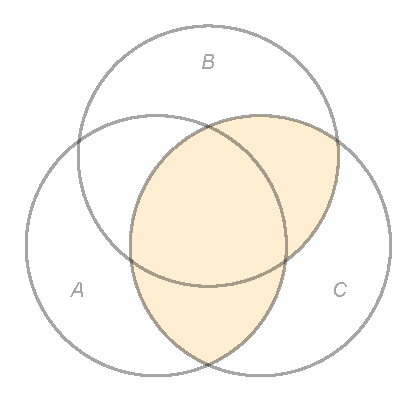
\includegraphics[width=0.2\textwidth]{images/venn1.pdf}}
            =
            \centerimage{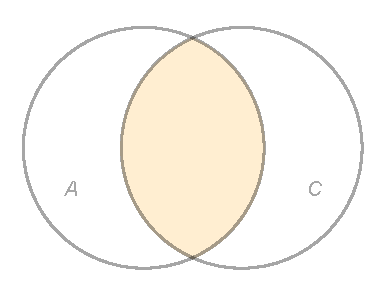
\includegraphics[width=0.2\textwidth]{images/venn2.pdf}}
            \cup
            \centerimage{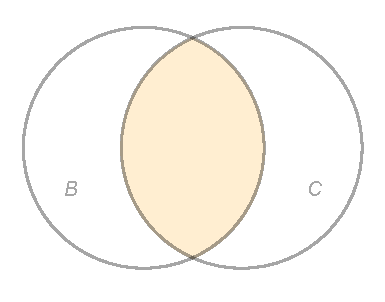
\includegraphics[width=0.2\textwidth]{images/venn3.pdf}}
            \]
            Demonstration of $A \cap \bigcup_{B \in \Gamma} B = \bigcup_{B \in \Gamma} (A \cap B)$, with $|\Gamma| = 3$.
            \[
            \centerimage{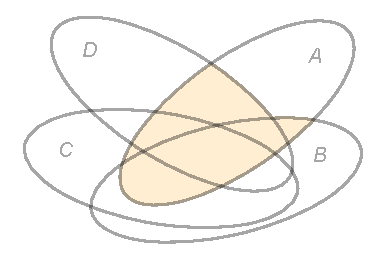
\includegraphics[width=0.2\textwidth]{images/venn4.pdf}} 
            =
            \centerimage{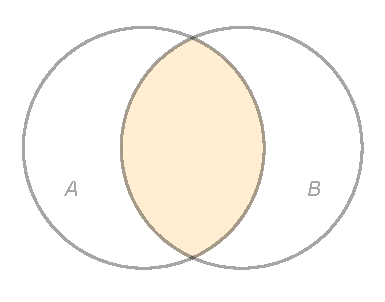
\includegraphics[width=0.2\textwidth]{images/venn5.pdf}} 
            \cup
            \centerimage{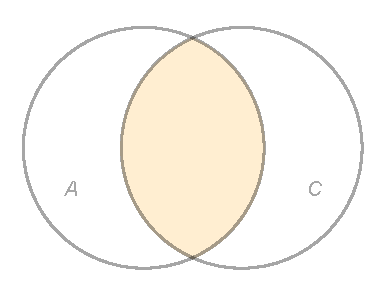
\includegraphics[width=0.2\textwidth]{images/venn6.pdf}} 
            \cup
            \centerimage{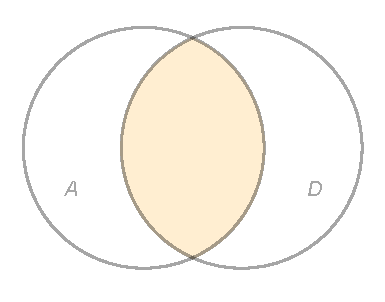
\includegraphics[width=0.2\textwidth]{images/venn7.pdf}} 
            \]
            Demonstration of $A \cup \bigcap_{B \in \Gamma} B = \bigcap_{B \in \Gamma} (A \cup B)$, with $|\Gamma| = 3$.
            \[
            \centerimage{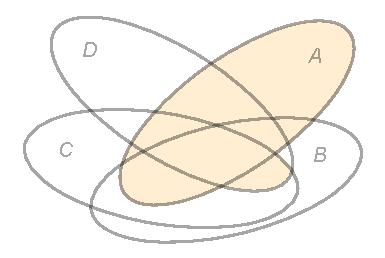
\includegraphics[width=0.2\textwidth]{images/venn11.pdf}} 
            =
            \centerimage{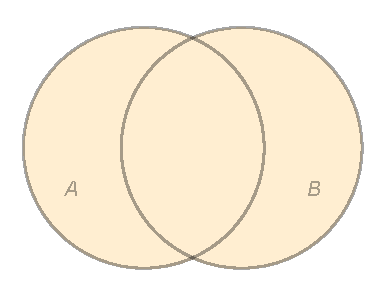
\includegraphics[width=0.2\textwidth]{images/venn8.pdf}} 
            \cap
            \centerimage{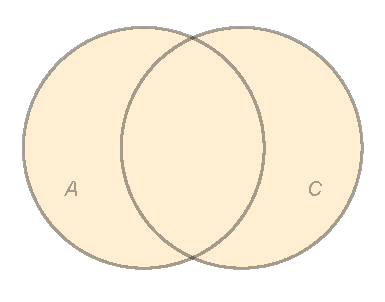
\includegraphics[width=0.2\textwidth]{images/venn9.pdf}} 
            \cap
            \centerimage{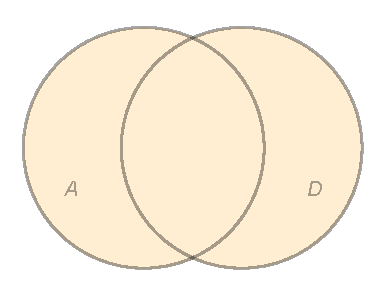
\includegraphics[width=0.2\textwidth]{images/venn10.pdf}} 
            \]
            
			\end{proof}
\begin{minorEx}[Riddle]%1.9
    Generalize Theorem 1.L to the case of arbitrary collections of sets.
\end{minorEx}
Let $A$ be a set and let $\Gamma$ be a set consisting of sets, then we have

$$A \cap  \bigcup_{B\in \Gamma} B = \bigcup_{B\in \Gamma} (A \cap B)\text{  and  } A \cup \bigcap_{B\in \Gamma} B = \bigcap_{B\in \Gamma} (A \cup B)$$
\begin{proof}
    See 1.N
\end{proof}
            
\begin{majorEx}[Yet Another Pair of Distributivities]%1.N 
Let $A$ be a set and let $\Gamma$ be a set consisting of sets, then we have

	$$A \cap  \bigcup_{B\in \Gamma} B = \bigcup_{B\in \Gamma} (A \cap B)\text{  and  } A \cup \bigcap_{B\in \Gamma} B = \bigcap_{B\in \Gamma} (A \cup B)$$
\end{majorEx}
\begin{proof}
	We will first show that $A \cap \bigcup_{B\in \Gamma} B = \bigcup_{B\in \Gamma} (A \cap B)$ using double containment. 
    
    First let $x \in A \cap \bigcup_{B\in \Gamma} B$ be arbitrary. We see that $$x \in A \land x\in B$$ for some $B \in \Gamma$. 
    We thus know that for some $B$, $$x\in (A \cap B)$$ 
    We now can see that as $$\bigcup_{B\in \Gamma} (A \cap B)$$ contains every $(A \cap B)$, we know that $$x \in \bigcup_{B\in \Gamma} (A \cap B)$$ 
    As $x$ was arbitrary, we know that $$A \cap \bigcup_{B\in \Gamma} B \subseteq \bigcup_{B\in \Gamma} (A \cap B)$$. 
    
    We now let $x \in \bigcup (A \cap B)$ be arbitrary. 
    We see that $$x \in A \land x \in B$$ for some $B\in \Gamma$.
    We also see that as $B\in \Gamma$, that $$B \subset \bigcup_{B\in \Gamma} B$$ and thus $x \in A \land x \in \bigcup_{B\in \Gamma}$.
    We now can see that this only holds if $$x \in A \cap \bigcup_{B\in \Gamma}$$ and thus as $x$ was arbitrary $$A \cap \bigcup_{B\in \Gamma} B \supseteq \bigcup_{B\in \Gamma} (A \cap B)$$. 
    We now can see by double containment, that $A \cap \bigcup_{B\in \Gamma} B = \bigcup_{B\in \Gamma} (A \cap B)$.
    
    We will now show that $$A \cup \bigcap_{B\in \Gamma} B = \bigcap_{B\in \Gamma} (A \cup B)$$ by double containment.
    
    We first let $x \in A \cup \bigcap_{B\in \Gamma} B$ be arbitrary.
   	We see that $$x \in A \lor x \in \bigcap_{B\in \Gamma} B$$ 
    We now suppose that $x \in A$. We would then see that $x \in A \cup B$ for any $B$, and thus $$x \in \bigcap_{B\in \Gamma} (A \cap B)$$
    
    Now suppose that $x \notin A$. We would then see that $$x \in \bigcap_{B\in \Gamma} B$$ and if $x$ is in some $B$, we know that it would also be in $A \cup B$, so thus, we would know that $$x \in \bigcap_{B\in \Gamma} (A \cup B)$$
    
    As $x$ was arbitrary, we know that 
    $$A \cup \bigcap_{B\in \Gamma} B \subseteq \bigcap_{B\in \Gamma} (A \cup B)$$
    
    We now let $x \in \bigcap_{B\in \Gamma} (A \cup B)$ be arbitrary. 
    We see that $x \in A$ or $x \in B$ for every $B \in \Gamma$. 
    Suppose $x \in A$. We would then see that $x \in A \cup \bigcap_{B\in\Gamma} B$ as $x \in A$. 
    Now, suppose that $x \notin A$ we would then have that $x \in \bigcap_{B\in\Gamma} B$ as $x \in \bigcap_{B\in\Gamma} (A \cap B)$, and $x \notin A$. We thus see that as $x$ was arbitrary, that $$A \cup \bigcap_{B\in \Gamma} B \supseteq \bigcap_{B\in \Gamma} (A \cup B)$$.
    
    and thus 
    $$A \cup \bigcap_{B\in \Gamma} B = \bigcap_{B\in \Gamma} (A \cup B)$$
    We can now see that
    
    $$A \cap  \bigcup_{B\in \Gamma} B = \bigcup_{B\in \Gamma} (A \cap B)\text{  and  } A \cup \bigcap_{B\in \Gamma} B = \bigcap_{B\in \Gamma} (A \cup B)$$
    
\end{proof}
\subsection{Different Differences}%1'12
			\begin{minorEx}%1.10
            Prove that for any two sets $A$ and $B$ their union $A \cup B$ is the union of the following three sets: $A \setminus B$, $B \setminus A$, and $A \cap B$, which are pairwise disjoint.
            \begin{proof}Let $A$, $B$ and $C$ be arbitrary sets. For an arbitrary value $a$, $a \in A \cup B$ iff $a \in A$ or $a \in B$. This is equivalent to $a \in A \cup B$ iff one of the three following conditions are met; $a \in A$ and $a \not \in B$, $a \not \in A$ and $a \in B$, or $a \in A$ and $a \in B$. \newline $a \in A \setminus B$ iff $a \in A$ and $a \not \in B$, $a \in B \setminus A$ iff $a \not \in A$ and $a \in B$, and $a \in A \cap B$ iff $a \in A$ and $a \in B$. So $a$ is in the union of these sets iff it meets one of those criteria by the definition of union. These criteria are the same as those enumerated about for $A \cup B$. Since $a$ was arbitrary, these sets must be the same.
            
            \end{proof}
            \end{minorEx}
            \begin{minorEx} % 1.11
            Prove that $A \setminus (A \setminus B) = A \cap B$ for any sets $A$ and $B$.
            \begin{proof}
            Let $x \in A \setminus (A \setminus B)$, by definition of set difference, we have $x \in A and x \not\in A \setminus B$. $x \not\in A \setminus B$ is the same as $x \in  (A \setminus B)^c$ which is equal to $B \cup A^c$. By distribution rule, $(A \cap (A^c \cup B)) = (A \cap A^c) \cup (A \cap B) = A \cap B$, so $x \in A \cap B$ and we have $A \setminus (A \setminus B) \subset A \cap B$. Since this process is reversible, we have $A \cap B  \subset A \setminus (A \setminus B)$, and we have: $$A \setminus (A \setminus B) = A \cap B$$
            \end{proof}
            \end{minorEx}

            \begin{minorEx} % 1.12
            Prove that $A \subset B$ if and only if $A \setminus B = \emptyset$.
            \end{minorEx}
            \begin{proof}
            We have $A \subset B$ if and only if there does not exist an $x \in A$ with $x \notin B$; which holds if and only if it is not the case that $A \setminus B \ne \emptyset$, which holds if and only if $A \setminus B = \emptyset$.
			\end{proof}
            
            \begin{minorEx}%1.13
            Prove that $A\cap (B \setminus C) =A\cap B \setminus A\cap C$ for any sets A,B, and C.
             \end{minorEx}
   	\begin{proof}
            We will show this by using double containment. 
            Let $x\in (A \cap (B \setminus C )$ be arbitrary. 
            We see that $x$ is in $A$, and in $B$, but not in $C$ and thus $x \in (A \cap B)$, and as $x$ is not in $C$, that $x\notin (A\cap C)$. We thus see that $x \in (A \cap B) \setminus (A \cap C)$.
            We thus see that as $x$ is arbitrary, we know that $A\cap (B \setminus C) \subseteq A\cap B \setminus A\cap C$.
            We now let $x \in (A \cap B) \setminus (A \cap C)$. 
            We see because of this, that $x$ is in $A$ and $B$, but that $x$ is not in $A$ and $C$.We thus know that $x \in A$, and because $x$ is in $A$, and $x$ is in $B$, but $x$ is not in $A$ and $C$, that $x$ is not in $B$ and $C$, and thus $x\in (B\setminus C)$. We thus see that $x \in A \cap (B \setminus C)$
            
	\end{proof}
    
    \begin{minorEx}%1.14
    Prove that for any sets $A$ and $B$ we have $$A \vartriangle B = (A \cup B) \setminus (A \cap B)$$
    \begin{proof}
    Let $A$ and $B$ be arbitrary sets. $A \vartriangle B$ denotes the set of values $a$ for which it is true either that $a \in A$ and $a \not \in B$ or $a \not \in A$ and $a \in B$. $(A \cup B) \setminus (A \cap B)$ denotes the set of values $b$ for which $b \in A \cup B$ and $b \not \in A \cap B)$. We then know $(A \cup B) \setminus (A \cap B)$ denotes the set of values $b$ for which $b \in A$ or $b \in B$ and $b \not \in A \cap B$. This is the same as the set of values $b$ for which $b$ belongs to exactly one of $A$ or $B$, i.e. the set of values for which it is true either that $b \in A$ and $b \not \in B$ or $b \not \in A$ and $b \in B$. We then have the exact same characterizations of $A \vartriangle b$ and $(A \cup B) \setminus (A \cap B)$, so the sets are the same.
    \end{proof}
    \end{minorEx}
    
    \begin{minorEx} % 1.15
    [Associativity of Symmetric Difference.] Prove that for any sets $A, B$ and $C$ we have $$(A \vartriangle B) \vartriangle C = A \vartriangle (B \vartriangle C)$$
    \end{minorEx}
    \begin{proof}
    To prove this equation we need to reinterpret the formula.
    
    LHS = 
    \begin{align*}
     & (A \vartriangle B) \vartriangle C \\
    =& ((A \cup B) \setminus (A \cap B)) \cup C \setminus ((A \cup B) \setminus ((A \cap B)) \cap C) \\
    =& A \cup B \cup C \setminus (A \cap B) \setminus (((A \cup B) \cap C) \setminus A \cap B \cap C) \\
    =& A \cup B \cup C \setminus (A \cap B) \setminus (((A \cap C) \cup (B \cap C) \setminus A \cap B \cap C)\\
    =& A \cup B \cup C \setminus ((A \cap B) \cup (A \cap C) \cup (B \cap C) \setminus A \cap B \cap C))\\
    \end{align*}
    
    RHS:
    \begin{align*}
    =& (A \vartriangle (B \vartriangle C)\\
    =& A \vartriangle (B \cup C \setminus B \cap C)\\
    =& A \cup (B \cup C \setminus B \cap C) \setminus A \cap (B \cup C \setminus B \cap C)\\
    =& (A \cup B \cup C \setminus B \cap C) \setminus (A \cap (B \cup C)) \setminus (A \cap B \cap C)\\
    =& A \cup B \cup C \setminus (((B \cap C) \cup (A \cap B) \cup (A \cap C)) \setminus (A \cap B \cap C)) = LHS\\
    \end{align*}
    We have: $$(A \vartriangle B) \vartriangle C = A \vartriangle (B \vartriangle C)$$
    \end{proof}
    
    \begin{minorEx}%1.16
    Riddle. Find a symmetric definition of the symmetric difference $(A \vartriangle B) \vartriangle C$ of three sets and generalize it to arbitrary finite collections of sets.
   	\end{minorEx}
    \begin{proof}
    We will start with the definition of symetric  difference for three sets. By the definition of symmetric difference of two sets, we can see that the symmetric difference between two sets is the result of removing their intersection from their union. We can then see that by iteratively applying this definition to a set C, that we have that all the elements of A, B, and C that don't belong another set are are included, that all the elements which belong to 2 sets are excluded, and all the elements which belong to both A, B, and C are included. From this, we can see that for 3 sets, the symmetric difference is composed of all elements which belong to an odd number of sets. By continuing to apply the symmetric diffence opperator, we would see that this remains to be the pattern, and thus the general pattern for the definition of symmetric difference will be the collection of elements of all sets which belong to an odd number of sets.
    \end{proof}
    \begin{minorEx}[Distributivity]%1.17
    Prove that $(A \vartriangle B) \cap C = (A \cap C) \vartriangle (B \cap C)$ for any sets $A$,$B$ ,and $C$
   	\end{minorEx}
    \begin{proof}
    Let $A$, $B$, and $C$ be arbitrary sets. We will show $(A \vartriangle B) \cap C = (A \cap C) \vartriangle (B \cap C)$ by double containment.
    
    We first let $x \in (A \vartriangle B) \cap C$ be arbitrary. We can see that $x\in C$ and $x\in (A \vartriangle B)$ by the properties of intersection. Because $x\in (A \vartriangle B)$, we know that $x \in A$ but $x \notin B$ or $x \in A$ but $x \notin B$. We thus know that $x\in C$ and $x\in A$, but $x\notin B$ or $x\in C$ and $x\in B$, but $x \notin A$. We can see that this is true if and only if $x \in (C \cap A) \setminus B \cup (C \cap B)\setminus A$, and thus $x \in (A \cap C) \vartriangle (B \cap C)$. As $x$ was arbitrary, we can see that $(A \vartriangle B) \cap C \subseteq (A \cap C) \vartriangle (B \cap C)$.
    
    We now let $x \in (A \cap C) \vartriangle (B \cap C)$ be arbitrary. We can see that $x \in (A \cap C)$, but $x\notin (B \cap C)$ or $x\in (B \cap C)$ but $x\notin (A \cap C)$. We thus can see that equivalently, $x \in A$ and $x\in C$ but $x\notin (B \cap C)$ or $x \in B$ and $x\in C$ but $x\notin (A \cap C)$. We can see that in every case that $x \in C$, and thus $x\in C$ and $x \in A$ but $x\notin B$, or $x \in B$ but $x\notin A$. We can see that this is equivilent to $x \in C \cap ((A\setminus B) \cup (B \setminus A ))$, and by the definition of symmetric difference, we can see that $x \in (A \vartriangle B) \cap C$. As $x$ was arbitrary, we can now see that $(A \vartriangle B) \cap C \supseteq (A \cap C) \vartriangle (B \cap C)$, and thus $(A \vartriangle B) \cap C = (A \cap C) \vartriangle (B \cap C)$
    \end{proof}
    \begin{minorEx}%1.18
    Does the following inequality hold true for any sets $A$, $B$, and $C$? $$(A \vartriangle B) \cup C = (A \cup C) \vartriangle (B \cup C)$$
    \begin{proof}
    For any sets $A$, $B$, $C$ where $C \subset A \cup B$, $(A \vartriangle B) \cup C = (A \cup C) \vartriangle (B \cup C)$.
    \end{proof}
    \end{minorEx}
            
%		\section{Topology on a Set}
%			\subsection{Definition of Topological Space}
%			\subsection{Simplest Examples}
%			\subsection{The Most Important Example: Real Line}
%			\subsection{Additional Examples}
%			\subsection{Using New Words: Points, Open Sets, Closed Sets}
%			\subsection{Set-Theoretic Digression: De Morgan Formulas}
%			\subsection{Properties of Closed Sets}
%			\subsection{Being Open or Closed}
%			\subsection{Characterization of Topology in Terms of Closed Sets}
%			\subsection{Neighborhoods}
%			\subsection{Open Sets on a Line}
%			\subsection{Cantor Set}
%			\subsection{Topology and Arithmetic Progressions}
%		\section{Bases}
%			\subsection{Definition of Base}
%			\subsection{When a Collection of Sets is a Base}
%			\subsection{Bases for Plane}
%			\subsection{Subbases}
%			\subsection{Infiniteness of the Set of Prime Numbers}
%			\subsection{Hierarchy of Topologies}
%		\section{Metric Spaces}
%			\subsection{Definition and First Examples}
%			\subsection{Further Examples}
%			\subsection{Balls and Spheres}
%			\subsection{Subspaces of Metric Spaces}
%			\subsection{Suprising Balls}
%			\subsection{Segments (What is Between)}
%			\subsection{Bounded Sets and Balls}
%			\subsection{Norms and Normed Spaces}
%			\subsection{Metric Topology}
%			\subsection{Openness and Closedness of Balls and Spheres}
%			\subsection{Metrizable Topological Spaces}
%			\subsection{Equivalent Metrics}
%			\subsection{Operations with Metrics}
%			\subsection{Distances between Points and Sets}
%			\subsection{Distances between Sets}
%			\subsection{Ultrametrics and $p$-Adic Numbers}
%			\subsection{Asymetrics}
%		\section{Subspaces}
%			\subsection{Topology for a Subset of a Space}
%			\subsection{Relativity of Openness and Closedness}
%			\subsection{Agreement on Notation for Topological Spaces}
%		\section{Position of a Point with Respect to a Set}
%			\subsection{Interior, Exterior, and Boundary Points}
%			\subsection{Interior and Exterior}
%			\subsection{Closure}
%			\subsection{Closure in Metric Space}
%			\subsection{Boundary}
%			\subsection{Closure and Interior with Respect to a Finer Topology}
%			\subsection{Properties of Interior and Closure}
%			\subsection{Compositions of Closure and Interior}
%			\subsection{Sets with Common Boundary}
%			\subsection{Convexity and $\text{Int}, \text{Cl}$, and \text{Fr}}
%			\subsection{Characterization of Topology by Operations of Taking Closure and Interior}
%			\subsection{Dense Sets}
%			\subsection{Nowhere Dense Sets}
%			\subsection{Limit Points and Isolated Points}
%			\subsection{Locally Closed Sets}
%		\section{Ordered Sets}
%			\subsection{Strict Orders}
%			\subsection{Nonstrict Orders}
%			\subsection{Relation between Strict and Nonstrict Order}
%			\subsection{Cones}
%			\subsection{Position of an Element with Respect to a Set}
%			\subsection{Linear Orders}
%			\subsection{Topologies Determined by Linear Order}
%			\subsection{Poset Topology}
%			\subsection{How to Draw a Poset}
%		\section{Cyclic Orders}
%			\subsection{Cyclic Orders in Finite Sets}
%			\subsection{Cyclic Orders in Infinite Sets}
%			\subsection{Topology of Cyclic Order}
%	\chapter{Continuity}
%	\setcounter{section}{8} %needed to fix counters to match the text
%		\section{Set-Theoretic Digression: Maps}
%			\subsection{Maps and Main Classes of Maps}
%		\section{Continuous Maps}
%		\section{Homeomorphisms}
%	
%	\chapter{Topological Properties}
%	\setcounter{section}{11} %needed to fix counters to match the text
%		\section{Connectedness}
%		\section{Applications of Connectedness}
%		\section{Path Connectedness}
%		\section{Separation Axioms}
%		\section{Countability Axioms}
%		\section{Compactness}
%		\section{Sequential Compactness}
%		\section{Local Compactness and Paracompactness}
%	
%	\chapter{Topological Constructions}
%	\setcounter{section}{19} %needed to fix counters to match the text
%		\section{Multiplication}
%		\section{Quotient Spaces}
%		\section{Zoo of Quotient Spaces}
%		\section{Projective Spaces}
%		\section{Finite Topological Spaces}
%		\section{Spaces of Continuous Maps}
%	
%	\chapter{Topological Algebra}
%	\setcounter{section}{25} %needed to fix counters to match the text
%		\section{Generalities on Groups}
%		\section{Topological Groups}
%		\section{Constructions}
%		\section{Actions of Topological Groups}
%\part{Elements of Algebraic Topology}
%	
%	\chapter{Fundamental Group}
%	\setcounter{section}{29} %needed to fix counters to match the text
%		\section{Homotopy}
%		\section{Homotopy Properties of Path Multiplication}
%		\section{Fundamental Group}
%		\section{The Role of Base Point}
%	
%	\chapter{Covering Spaces and Calculation of Fundamental Groups}
%	\setcounter{section}{33} %needed to fix counters to match the text
%		\section{Covering Spaces}
%		\section{Theorems on Path Lifting}
%		\section{Calculations of Fundamental Groups by Using Universal Coverings}
%
%%
%%
%%	
%	\begin{thebibliography}{1}
%	  	\bibitem{viro} O. Ya. Viro, O. A. Ivanov, N. Yu. Netsvetaev, V. M. Kharlamov. {\em Elementary Topology Problem Textbook}. Retrieved August 10, 2016: \url{http://www.pdmi.ras.ru/~olegviro/topoman/eng-book-nopfs.pdf}.
%	\end{thebibliography}
\end{document}